\documentclass[12pt,a4paper]{report}

%adjust your page margins here
\usepackage[top=0.70in, bottom=0.70in, left=0.8in,right=0.80in]{geometry} % setting the page alignment with this package
\usepackage[pdftex]{graphicx} %for embedding images
\usepackage[%dvips, % commented for pdflatex
bookmarks,  colorlinks=false]{hyperref} %for creating links in the pdf version and other additional pdf attributes, no effect on the printed document
\hypersetup{%
    pdfborder = {0 0 0}
}
\usepackage[final]{pdfpages} %for embedding another pdf, remove if not required
\usepackage{float} %used for figure placement with H as a parameter
\usepackage{hyperref}
\usepackage{pslatex} % for times new roman, old package, but works
\usepackage{array} % for making text bold in table
\usepackage{setspace}
\usepackage{float}
\usepackage{enumerate}
\usepackage{longtable}

\usepackage[font=small,labelfont=bf]{caption}
\def\figurename{\textbf{Figure }}

\usepackage{listings}
\usepackage{color}

\definecolor{dkgreen}{rgb}{0,0.6,0}
\definecolor{gray}{rgb}{0.5,0.5,0.5}
\definecolor{mauve}{rgb}{0.58,0,0.82}
 
\lstset{ %
  language=Java,                % the language of the code
  basicstyle=\footnotesize,           % the size of the fonts that are used for the code
  numbers=left,                   % where to put the line-numbers
  numberstyle=\tiny\color{gray},  % the style that is used for the line-numbers
  stepnumber=1,                   % each line is numbered
  numbersep=5pt,                  % how far the line-numbers are from the code
  backgroundcolor=\color{white},      % choose the background color. You must add \usepackage{color}
  showspaces=false,               % show spaces adding particular underscores
  showstringspaces=false,         % underline spaces within strings
  showtabs=false,                 % show tabs within strings adding particular underscores
  frame=single,                   % adds a frame around the code
  rulecolor=\color{black},        % if not set, the frame-color may be changed on line-breaks within not-black text (e.g. commens (green here))
  tabsize=2,                      % sets default tabsize to 2 spaces
  captionpos=b,                   % sets the caption-position to bottom
  breaklines=true,                % sets automatic line breaking
  breakatwhitespace=false,        % sets if automatic breaks should only happen at whitespace
  title=\lstname,                   % show the filename of files included with \lstinputlisting;
                                  % also try caption instead of title
  keywordstyle=\color{blue},          % keyword style
  commentstyle=\color{dkgreen},       % comment style
  stringstyle=\color{mauve},         % string literal style
  escapeinside={\%*}{*)},            % if you want to add a comment within your code
  morekeywords={*,...}               % if you want to add more keywords to the set
}

%For the header and footer
\usepackage{fancyhdr}
\fancypagestyle{plain}{%
\fancyfoot[L]{\emph{Department of Computer Engineering, SHORT NAME OF COLLEGE, Pune}} % except the center
\fancyfoot[R]{\thepage}
\renewcommand{\headrulewidth}{0.4pt}
\renewcommand{\footrulewidth}{0.4pt}
}

\pagestyle{fancy}

\rhead{\emph{NAME OF PROJECT}}

\fancyfoot[LO,LE]{\emph{Department of Computer Engineering, SHORT NAME OF COLLEGE, Pune}}
\cfoot{}
\fancyfoot[RO, RE]{\thepage}
\renewcommand{\headrulewidth}{0.4pt}
\renewcommand{\footrulewidth}{0.4pt}
%For the header and footer Over

%Page Border
\usepackage{pgf}
\usepackage{pgfpages}

\pgfpagesdeclarelayout{boxed}
{
  \edef\pgfpageoptionborder{0pt}
}
{
  \pgfpagesphysicalpageoptions
  {%
    logical pages=1,%
  }
  \pgfpageslogicalpageoptions{1}
  {
    border code=\pgfsetlinewidth{2pt}\pgfstroke,%
    border shrink=\pgfpageoptionborder,%
    resized width=.95\pgfphysicalwidth,%
    resized height=.95\pgfphysicalheight,%
    center=\pgfpoint{.5\pgfphysicalwidth}{.5\pgfphysicalheight}%
  }%
}
\pgfpagesuselayout{boxed}
\setlength{\parindent}{1cm}
%GLOBAL SETTINGS OVER, DOCUMENT BEGINS
\begin{document}
\renewcommand\bibname{References}
\lhead{ }

%FROM HERE YOUR PAGES START GETTING ADDED

% includes the cover page
\newpage
\begin{center}
\thispagestyle{empty}
\Large{\textbf{A PROJECT REPORT\\ \large{ON}}}\\[0.7cm]
\LARGE{\textsc {\textbf{``NAME OF PROJECT''}}}\\[0.5cm]
\vspace{0.5cm}
\Large{\textbf{\\Submitted to}}
\LARGE{\textbf{\\UNIVERSITY OF PUNE\\}}
\vspace{1cm}
\Large{\textbf{\\In Partial Fulfilment of the Requirement for the Award of\\}}
\Large{\textbf{\\BACHELOR'S DEGREE IN\\COMPUTER ENGINEERING}}
\vspace{1cm}
\Large{\textbf{\\BY}}\\[0.5cm]
\begin{table}[h]
\centering
\Large{
\begin{tabular}{>{\bfseries}lc>{\bfseries}r}
GROUP MEMBER A & & ROLL NUMBER A\\GROUP MEMBER B & & ROLL NUMBER B\\GROUP MEMBER C & & ROLL NUMBER C\\GROUP MEMBER D & & ROLL NUMBER D\\
\end{tabular}}
\end{table}
\vspace{0.5cm}
\large{\textbf{UNDER THE GUIDANCE OF}}\\
\large{\textbf{PROF. GUIDE NAME}}\\
\vspace{1cm}
\large{\textbf{DEPARTMENT OF COMPUTER ENGINEERING}}\\
\Large{\textbf{NAME OF COLLEGE}}\\
\large{\textbf{LOCATION IN PUNE, PUNE - PINCODE}}
\large{\textbf{\\2012-2013}}\\
\vspace{1cm}
\Large{\textbf{AFFILIATED TO\\}}
\LARGE{\textbf{UNIVERSITY OF PUNE}}
\newpage
\end{center}
\newpage

\begin{titlepage}

\begin{center}

\textup{\small {\bf CSU498 Project} \\ Report}\\[0.2in]

% Title
\Large \textbf {<Title here>}\\[0.5in]

       \small \emph{Submitted in partial fulfillment of\\
        the requirements for the award of the degree of}
        \vspace{.2in}

       {\bf Bachelor of Technology \\in\\ Computer Science and Engineering}\\[0.5in]

% Submitted by
\normalsize Submitted by \\
\begin{table}[h]
\centering
\begin{tabular}{lr}\hline \\
Roll No & Names of Students \\ \\ \hline
\\
<Roll no here> & <Name here> \\
<Roll no here> & <Name here> \\ 
<Roll no here> & <Name here> \\ \\ \hline 
\end{tabular}
\end{table}

\vspace{.1in}
Under the guidance of\\
{\textbf{<Guide's name here>}}\\[0.2in]

\vfill

% Bottom of the page

\includegraphics[width=0.18\textwidth]{nitc-logo}\\[0.1in]
\Large{Department of Computer Science and Engineering}\\
\normalsize
\textsc{National Institute of Technology Calicut}\\
Calicut, Kerala, India -- 673 601 \\
\vspace{0.2cm}
Winter Semester 2013

\end{center}

\end{titlepage}

\newpage

% includes the certificate page
\newpage
\thispagestyle{empty}

\begin{center}

\huge{Department of Computer Science and Engineering}\\[0.5cm]
\normalsize
\textsc{National Institute of Technology Calicut}\\[2.0cm]

\emph{\LARGE Certificate}\\[2.5cm]
\end{center}
\normalsize This is to certify that this is a bonafide record of the project presented by the students whose names are given below during <Monsoon/Winter and Year here> in partial fulfilment of the requirements of the degree of Bachelor of Technology in Computer Science and Engineering.\\[1.0cm]

\begin{table}[h]
\centering
\begin{tabular}{lr}
Roll No & Names of Students \\ \\ \hline
\\
<Roll no here> & <Name here> \\ 
<Roll no here> & <Name here> \\
<Roll no here> & <Name here> \\
\end{tabular}
\end{table}

\vfill


% Bottom of the page
\begin{flushright}
<Guide name here>\\
(Project Guide)\\[1.5cm]
<Coordinator name here>\\
(Course Coordinator)\\
\end{flushright}

\begin{flushleft}
Date:
\end{flushleft}
 
\newpage

% includes the acknowledgements page
\begin{center}
\thispagestyle{empty}
\LARGE{\textbf{Acknowledgements}}\\[1cm]
\end{center}
\linespread{1.13}
\large{\paragraph{}We are profoundly grateful to \textbf{Prof. GUIDE NAME} for his expert guidance
and continuous encouragement throughout to see that this project rights its
target since its commencement to its completion.}
\large{\paragraph{}We would like to express deepest appreciation towards \textbf{Dr. PRINCIPAL NAME},
Principal, NAME OF COLLEGE, \textbf{Prof. HOD NAME}, 
Head of Department of Computer Engineering and \textbf{Prof. PROJECT COORDINATOR NAME}, Project Coordinator whose
invaluable guidance supported us in completing this project.}
\large{\paragraph{}At last we must express our sincere heartfelt gratitude to all the staff members
of Computer Engineering Department who helped me directly or indirectly during this course of work.}
\begin{flushright}
{
GROUP MEMBER A\\
GROUP MEMBER B\\
GROUP MEMBER C\\
GROUP MEMBER D
}
\end{flushright}
\newpage
 
\newpage

\vspace{2in}
\begin{abstract}

<Abstract here>

\end{abstract} 
 % adds the Research Methodology page
\newpage

%TABLE OF CONTENTS AND LIST OF FIGURES ARE AUTOMATICALLY ADDED BY FOLLOWING COMMANDS
%ADD FIGURE OF TABLES IF YOU NEED TO, CHECK DOCUMENTATION
\pagenumbering{roman} %numbering before main content starts


%To reset the Header & Footer for TOC and LOF
\pagestyle{empty}
\addtocontents{toc}{\protect\thispagestyle{empty}}
\tableofcontents % adds Index Page

\addtocontents{lof}{\protect\thispagestyle{empty}}
\listoffigures % adds List of Figures
\cleardoublepage

%And reset back the settings we choose for Header and Footer
\pagestyle{fancy}

\newpage
\pagenumbering{arabic} %reset numbering to normal for the main content

\chapter{Introduction}
\section{SECTION NAME}
\subsection{SUBSECTION NAME 1}
\paragraph{}WRITE HERE

\begin{figure}[H]
  \centering
    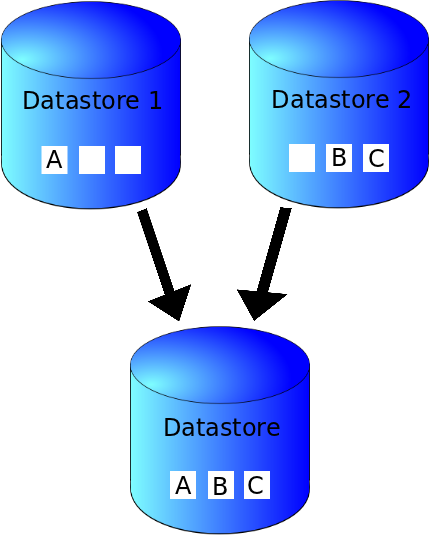
\includegraphics[height= 10cm, width=15cm]{project/images/data-sync}
  \caption{\textbf{IMAGE CAPTION}}
\end{figure}

\subsection{SUBSECTION NAME 2}
\paragraph{}WRITE HERE
 % adds the introduction page
\chapter{Literature Survey}
\section{SECTION NAME}
\paragraph{}WRITE HERE
\begin{enumerate}[a. ]
 \item ITEM 1
 \item ITEM 2
 \item ITEM 3
\end{enumerate} % adds the Literature Survey page
\chapter{Software Requirements Specification}
\section{SECTION NAME}
\subsection{SUBSECTION NAME}
\paragraph{} WRITE HERE.
\chapter{Requirement Analysis}
\section{SECTION NAME}
\paragraph{} WRITE HERE.
\chapter{System Design}
\section{SECTION NAME}
\paragraph{} WRITE HERE.
\chapter{System Testing}
\paragraph{} WRITE HERE.
\section{Test Cases and Test Results}
\begin{longtable}{ | p{1cm} | p{3.5cm} | p{4cm} | p{4cm} | p{4cm} |}
      \hline
      \textbf{Test ID} & \textbf{Test Case Title} & \textbf{Test Condition} & \textbf{System Behavior} & \textbf{Expected Result}\\
      \hline
      T01 & AAAA & BBBB & CCCC & DDDD\\
      \hline
      T02 & AAAA & BBBB & CCCC & DDDD\\
      \hline
      T03 & AAAA & BBBB & CCCC & DDDD\\
      \hline
\end{longtable}

\textbf{Note: Testing should be performed manually}
\chapter{Project Planning}
\section{SECTION 1}
\paragraph{} WRITE HERE.

\chapter{Implementation}
\paragraph{}WRITE HERE, PARAGRAPH 1.
\paragraph{}WRITE HERE, PARAGRAPH 2.

\begin{figure}[H]
  \centering
    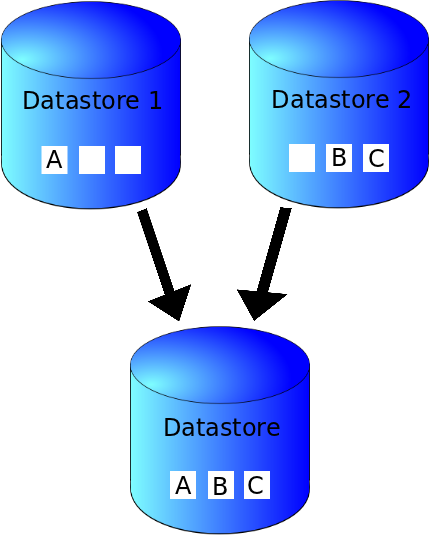
\includegraphics[scale=0.5]{project/images/data-sync}
  \caption{\textbf{IMAGE CAPTION}}
\end{figure}

\begin{lstlisting}
  PASTE YOUR CODE HERE
\end{lstlisting}
\newpage

 % adds the Project Design
\chapter{Screenshots of Project}
\section{SECTION NAME}
\vspace{2cm}
\begin{figure}[H]
  \centering
    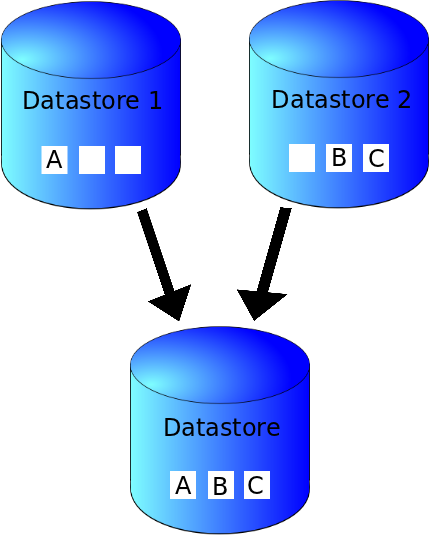
\includegraphics[height= 11cm, width=17cm]{project/images/data-sync}
\end{figure}
\newpage
\begin{figure}[H]
  \centering
    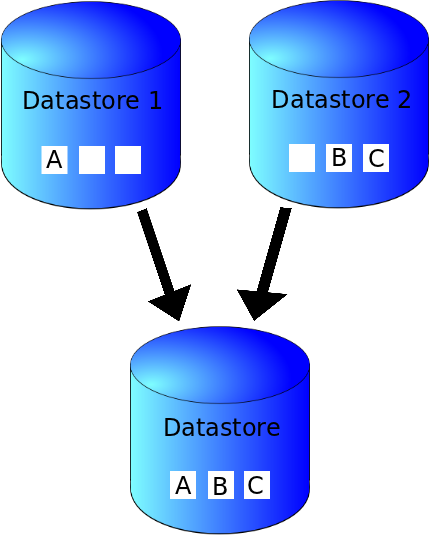
\includegraphics[height= 11cm, width=17cm]{project/images/data-sync}
\end{figure}
\vspace{1cm}
\begin{figure}[H]
  \centering
    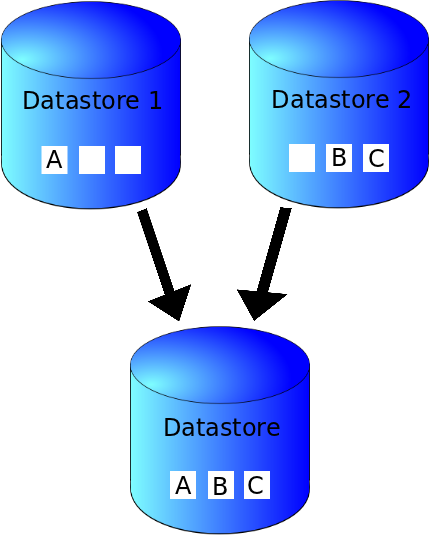
\includegraphics[height= 11cm, width=17cm]{project/images/data-sync}
\end{figure}
\chapter{Conclusion}

<Conclusion here>
 % adds the Scheduling and Planning page
\addcontentsline{toc}{chapter}{References}
\begin{thebibliography}{99}
\bibitem{WRITE A SHORT-NAME WITHOUT SPACE} \emph{NAME OF IEEE PAPER}; NAME OF AUTHORS
\bibitem{WRITE A SHORT-NAME WITHOUT SPACE} \url{http://EXAMPLE.com}
\end{thebibliography} % adds the References page

\end{document}